\subsection{Definícia a reprezentácia grafov}

Grafy slúžia ako model objektov a ich vzájomných vzťahov. Skladajú sa z vrcholov (uzlov) a z hrán. V práci budeme označovať graf ako G = (V, E), pričom V označuje množinu vrcholov a E označuje množinu hrán. Pri vizualizácií budeme vrchold zobrazovať ako bod či kruh a hranu ako úsečku, pričom jej konce budú vždy v nejakom vrchole. Dva vrcholy grafu môžu byť spojené jednou alebo viacerými hranami. V prípade, že dva vrcholy spája viac ako jedna hrana, hovoríme o viacnásobnej hrane. Hrana môže viesť taktiež z vrcholu do samého seba, v tom prípade hovoríme o hrane ako o slučke. Podmnožinou grafu označujeme ľubovoľnú podmnožinu hrán a vrcholov \citep{markovsovadynamika}. Rozlišujeme viacero typov grafov, ktoré sa rozlišujú na základe veľkosti, spôsobu vytvorenia, vlastností hrán, vlastností vrcholov a iných rôznych atribútov. V nasledujúcich častiach si spomenieme základné a pre nás potrebné rozdelenia, ktoré neskôr použijeme. \\

Na reprezentáciu grafu sa dajú použiť viaceré spôsoby, dve z najtypickejších sú incidenčná matica a matica susedností. V incidenčnej matice označujú riadky uzly a stĺpce hrany. Prvok matice nadobúda hodnotu rôznu od nuly práve vtedy, keď je daná hrana incidentná s daným uzlom, inak povedané, ak do uzla daná hrana vchádza či vychádza. Riadky a stĺpce matice susednosti fungujú iným spôsobom. Aj riadky, aj stĺpce reprezentujú vrcholy, pričom prvky matice reprezentujú počty hrán medzi jednotlivými dvojicami uzlov \citep{markovsovadynamika}.  V prípade neorientovaných grafov môžeme v matici susedností pozorovať vlastnosť symetrie okolo hlavnej diagonály \citep{cormen2009introduction}, toto však nemusí platiť pri orientovaných grafoch. Graf neobsahujúci slučky zase neobsahuje na diagonále hodnoty iné od nuly. Ako príklad uvádzame tieto reprezentácie pre obrázok \ref{fig:img1} nižšie.

\[ IM= \left( \begin{array}{cccc}
1 & 1 & 0 & 0\\
0 & 0 & 1 & 1\\
1 & 0 & 1 & 0\\
0 & 1 & 0 & 1\\
\end{array} \right)
%
MS= \left( \begin{array}{cccc}
0 & 0 & 1 & 1 \\
0 & 0 & 1 & 1\\
1 & 1 & 0 & 0\\
1 & 1 & 0 & 0\\
\end{array} \right)
\label{eq:matrices}
\]



\begin{figure}[H]
    \centering
    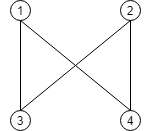
\includegraphics[width=0.5\textwidth]{subsections/images/graph_matrix.png}
    \caption{Príklad grafu}
    \label{fig:img1}
\end{figure}


